We test the four hypotheses system by system, from the toy networks, where parts can be new to the system, to the pretrained models, where they are new only to the probe. Each system answers one question about the gap between behavior and state, and Table~\ref{tab:remedies} collects the repairs. Figure~\ref{fig:ladder} summarizes the first three hypotheses.


\subsection{Glyph networks keep new glyphs their decoders cannot draw}
\label{app:states}

Glyph networks come first because they are the one setting where a glyph can be new to the network itself. Only here can we tell whether a decoder that fails on a new glyph has lost the glyph or merely left it unread.

\textbf{Glyph networks act weakly.} Every architecture reproduces new pairs of training glyphs with output $R^2$ between 0.85 and 1.00, except the transformer trained on eight glyphs. New glyphs separate the networks by vocabulary. At $m = 64$, their output on new glyphs rises from 0.20--0.34 at $V = 8$ to 0.85--0.91 at $V = 64$ (Figure~\ref{fig:strong}b).

\textbf{Their states keep the new glyphs.} One MLP trained on 8 glyphs renders five wholes of new glyphs with a mean $R^2$ of $-0.15$, whereas a linear probe of its state recovers them with 0.76 (Figure~\ref{fig:strong}a shows four of them). Across the MLP, CNN and role--filler networks, the broad probe recovers 0.83--0.86 at $V = 8$ and 0.89 at $V = 64$, or $\kappa = 0.73$ and 0.83. The glyph's part vector carries the glyph, because a linear map of it recovers the latent with $R^2 = 0.92$. The transformer is the exception, at 0.59 for $V = 8$.

\textbf{The decoders behave like probes fitted on their vocabulary.} The vocabulary probe recovers only 0.23--0.29 of new glyphs at $V = 8$, and it tracks each network's own output better than the broad probe does. Proposition~\ref{prop:span} predicts this behavior, and it also predicts that distinct parts drive the decoder's reach. With 140 training pairs, moving from 16 to 64 glyphs raises the output on new glyphs from 0.47--0.64 to 0.81--0.82.

\textbf{A new decoder reads the state.} We freeze the encoder of each network trained on 8 glyphs and train a new decoder of the same architecture on wholes of 64 other glyphs. The new decoder renders new glyphs at 0.75, against 0.25 for the network's own decoder and 0.88 for networks trained end to end on 64 glyphs. Across architectures and vocabularies, the broad probe of a frozen encoder correlates with the output of its new decoder at $r = 0.87$, so recoverability predicts the procedures a state can support. Untrained encoders keep the glyphs almost as well and support an equally good new decoder (Section~\ref{sec:origins}), so in these small networks the gap sits in the decoder. Single glyphs teach the same lesson. Adding 64 other glyphs shown alone, each in one role with the other role blank, lets networks trained on all pairs of 8 glyphs render a new glyph alone with $R^2 = 0.88$, against $-0.30$ without them, and new pairs with 0.47, against 0.26.

\begin{figure}[t]
  \centering
  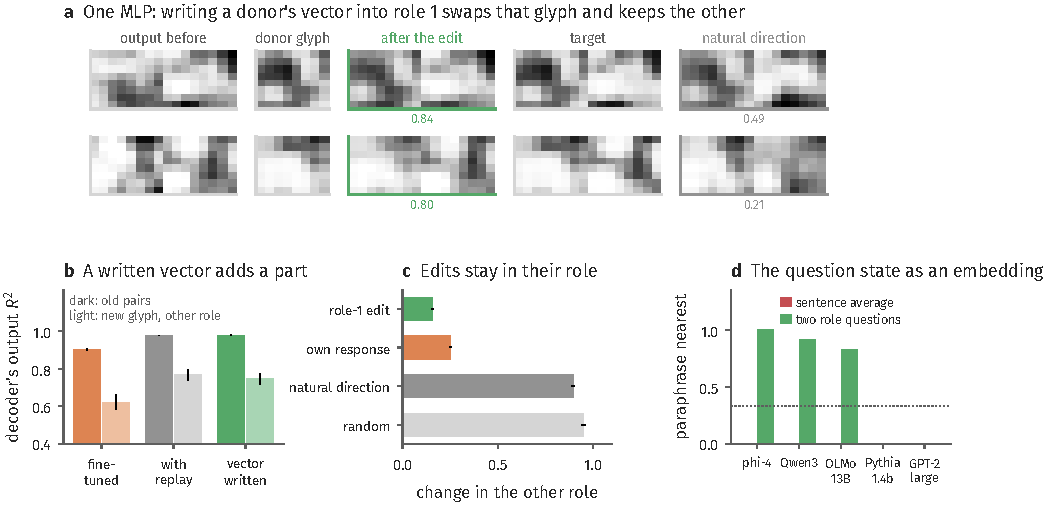
\includegraphics[width=\linewidth]{fig_decomp.pdf}
  \caption{\textbf{Procedures that read through role codes reuse the parts.} Role maps $h \approx c + B_1 e(x) + B_2 e(y)$, fitted on many glyphs, predict and edit states that each network's own decoder renders (\textsc{over}, $V = 64$). \textbf{a.} A code swap replaces the role-1 vector with a donor's vector, and the decoder renders the donor in role 1 while keeping the role-2 glyph. The natural direction $h(a', b') - h(a, b)$, scaled to the same norm, lands far from the target. Numbers give $R^2$ to the target. \textbf{b.} Writing a new glyph's vector through $B_2$ keeps old pairs (dark) and renders the new glyph in a role it never filled (light), with no gradient step, whereas fine-tuning damages both and replay needs stored data. \textbf{c.} A role-1 swap changes the role-2 half of the output less than other changes of the state do. \textbf{d.} In language models that answer by meaning, the state at two role questions places a sentence's converse paraphrase nearer than both role reversals, with no fitted probe, whereas the average over tokens never does; chance is $1/3$ (dotted). Means over 3--5 seeds, with standard errors.}
  \label{fig:decomp}
\end{figure}

\textbf{Swapping a role's vector changes one part.} Under \textsc{over}, the role residual $\delta$ is 0.02--0.04 for the MLP, CNN and role--filler networks and 0.06--0.13 for the transformer, so the states reach recoverability through shared role codes. A code swap writes a donor's vector into role 1, and the decoder renders the donor with $R^2 = 0.78$, against 0.81 when the network sees the donor itself (Figure~\ref{fig:decomp}a). The swap spills 0.16 into the untouched half of the output, against 0.90 for the natural direction $h(a', b') - h(a, b)$ (Figure~\ref{fig:decomp}c). The decoders therefore use the role codes, which answers the objection of \citet{fodor1990} for these systems. Under the non-additive \textsc{occlude}, $\delta$ rises to 0.11--0.22 and swaps spill 0.31.

\textbf{Written vectors add glyphs without forgetting.} We test additions twice. First, networks trained on 64 glyphs meet one new glyph in role~1 (Figure~\ref{fig:decomp}b). Fine-tuning on it damages the network, so the glyph in role~2 falls from 0.75 for the unmodified network to 0.62 and pairs of training glyphs fall from 0.98 to 0.90. Writing the glyph's vector into role~2 through $B_2$ takes no gradient step, so the old pairs stay at 0.98 while the decoder renders the glyph in a role it never filled at 0.75. Replay reaches 0.77, at the cost of stored data. Second, MLP, CNN and role--filler networks trained on 16 glyphs receive 32 new glyphs in sequence. Fine-tuning drops their old pairs to 0.18, as in catastrophic interference \citep{mccloskey1989}, whereas written vectors keep the old pairs at 0.99 and render each new glyph in a role it never filled at 0.71. Replay does better on the new glyphs, by 0.11--0.21, although it stores old data and takes gradient steps. A training objective that asks the state to give back many glyphs also helps the network's own decoder (Appendix~\ref{app:extra}).

\subsection{Recursive composers show the same gap at depth}
\label{app:depth}

Nesting is the capability that classical arguments for constituent structure lean on most \citep{fodor1988}, so we next ask whether the gap survives one level deeper than training.

\textbf{The decomposer fails beyond its training depths, and the root state does not.} Within its training depths, a recursive composer's own decomposer recovers new leaves almost perfectly for $w \ge 32$. At depth 3 it falls to $R^2 = 0.26$ at $w = 256$ after 6{,}000 steps, whereas a broad probe recovers the same leaves with 0.99 (Figure~\ref{fig:strong}c). At depths 4 and 5, which the composer never saw, the probe stays within 0.14 of the ceiling of Proposition~\ref{prop:depth}. HRR shows the same pattern by design. Recursive unbinding loses about $(2^n - 1)d/w$ of the variance to crosstalk and falls from 0.96 at depth 1 to $-0.13$ at depth 5, while a probe of the same state recovers the leaves exactly whenever $w \ge 2^n d$.

\textbf{Training at depth repairs the decomposer.} A decomposer that trains with its composer on trees of depth 3 to 5 recovers new leaves at 1.00, 1.00 and 0.97 at width 256, the values of the broad probe. Trained alone on the composer's states, the decomposer reaches only 0.74, 0.29 and 0.09, and no condition transfers to depth 6.

\subsection{Image encoders keep fixed places that their matching ignores}
\label{app:images}

The toy pattern would matter little if it vanished in models trained on the open world. Image--text encoders are a natural first test, because we score them by how well they match captions, a behavioral test of composition.

\textbf{Image encoders hold fixed places that their matching ignores.} CLIP-B/32, CLIP-H/14 and SigLIP prefer a caption that names the two new photographs over a caption with one wrong object, with accuracy 0.88--0.97. Against the caption with the two places swapped, however, they score 0.50--0.51, which is chance (Figure~\ref{fig:strong}d). Their quadrant states recover both photographs in their fixed places with $\kappa = 0.81$--$0.94$, and with 0.85--0.94 under \textsc{overlap}, against 0.29--0.72 for random weights across the encoders. The matching reads a single pooled embedding, and the average over patches, the closest state we probe, keeps far less of the places, at $\kappa = 0.17$--$0.49$ (Section~\ref{sec:origins}). Behavior agrees with the pooled state that the matching reads, and the recoverable state sits upstream, in the spatial map of the patch states. A matcher built on the quadrant states should close the gap for fixed layouts, and we leave that repair untested.

\textbf{Absolute positions carry most of these places.} A fixed quadrant ties each role to one location, so a probe can return the photographs by where they sit whether or not the state marks which one is the figure. To loosen this tie, we place both photographs at $64 \times 64$ pixels on one random row of a $448 \times 448$ canvas, at random horizontal positions, and the left photograph is the figure wherever the pair lands. With the same quadrant averages, part vectors and validation choices, the trained encoders recover both photographs in their roles with $\kappa = 0.24$ for CLIP-B/32, 0.42 for DINOv2-L and 0.45 for SigLIP, and a $4 \times 4$ grid of patch averages gives 0.18--0.49, against 0.81--0.93 for the same encoders under fixed quadrants. Random weights fall from 0.63--0.68 under fixed quadrants to $-0.17$ to $-0.71$, so their fixed-quadrant score came from location alone. The smaller photographs keep their identity, because features pooled within each photograph's box, taken in left-to-right order, still give 0.66--0.80. When the probe receives the two box features in random order and must find the figure itself, every encoder falls below zero, at $-0.08$ to $-0.17$. The trained encoders keep 0.18--0.49 of the relative places, and even this remainder may come from position, because a threshold on one photograph's horizontal position predicts the role with accuracy 0.84 and every encoder falls below zero when it must find the figure from the box features alone.

\subsection{Diffusion models keep fixed places that their own classifier ignores}
\label{app:diffusion}

Text-to-image diffusion models are the most cited case of machine composition after language models, and they supply an output of their own that reads the same canvases as the image encoders. A diffusion model scores a caption by how well it denoises an image under that caption, so the caption with the lower denoising error is the model's own choice \citep{li2023diffclassifier,clark2023diffclassifier}. We give Stable Diffusion 1.5 and SDXL the two-photograph canvases of Section~\ref{sec:images}, encoded by each model's autoencoder, and we compare captions over 25 timesteps from 50 to 950. The state is the denoiser's feature map from its middle and upsampling blocks, read with an empty caption and a fixed noise draw, and validation photographs choose the block and the timestep. SDXL runs at 512 pixels, below its native resolution.

\textbf{The model's own classifier ignores places.} Choosing by denoising error, SD 1.5 prefers the caption that names both photographs over a caption with one wrong object with accuracy 0.86--0.88, and SDXL with 0.69--0.71. Against the caption with the two places swapped, both models score 0.49--0.50, and no single timestep lifts either above 0.52. The denoising error sums over the whole map, and the next paragraph shows that the whole-map average of the features keeps little of the places.

\textbf{The denoiser's state keeps fixed places.} A linear probe of the denoiser's features, averaged within each quadrant, recovers both photographs in their fixed places with $\kappa = 0.70$ in SD 1.5 and 0.43 in SDXL (Figure~\ref{fig:ladder}). In SD 1.5 the score is 0.73 for \textsc{beside} and \textsc{above} and 0.66 for \textsc{overlap}. Averaged over the whole map, the same features give 0.13 and 0.05, so a reading that pools the whole map keeps almost none of the places. Behavior agrees with that low-recoverability reading, and the recoverable state sits upstream, in the spatial layout of the features. Under the relative places of Section~\ref{sec:images}, the places vanish from SD 1.5's state: quadrant averages give $\kappa = -0.06$ and the $4 \times 4$ grid gives $-0.14$. Box features in left-to-right order reach only 0.35, so the small photographs also lose much of their identity in the denoiser, and its places rest on fixed locations. SDXL remains untested under relative places.

\textbf{Training builds the places into the state.} Read against the trained model's part vectors, the same ones that the trained, random and latent comparison uses throughout, the autoencoder's latent, which is the denoiser's input, gives $\kappa = -0.48$ in SD 1.5 and $-0.47$ in SDXL, and the denoiser under random weights gives 0.12 and 0.09. Against the trained model's part vectors, training builds recoverability beyond the input and beyond random weights, as in the other pretrained models (Section~\ref{sec:origins}). As a stated caveat, a random denoiser read against its own part vectors reaches 0.80 and 0.83, because its vector for a single photograph keeps low-level detail that a linear probe matches easily.

\textbf{Generation ignores the relation as well.} We ask SD 1.5 for 150 pairs of new nouns in three relations, such as ``a cherry to the left of a tire'', in the canonical phrasing and in its converse, ``a tire to the right of a cherry'', with four seeds each, and we locate both objects with a detector \citep{liu2024groundingdino}. SD 1.5 often fuses the two objects or omits one, so about 200 images per relation and phrasing hold both objects as separate boxes. Among these, the figure lands in its place with accuracy 0.47--0.56 in every relation and phrasing, and the first-mentioned noun takes the first place equally often, at all three detector thresholds we tried. Under a shared seed, the two phrasings give the same layout for 0.63--0.75 of pairs, so the noise and the nouns set the layout and the relation word leaves it in place. SDXL at its native 1{,}024 pixels, with 50 pairs and two seeds per relation and phrasing, repeats the pattern for \textsc{above} and \textsc{left of}, at 0.46--0.55. For \textsc{on} it places the figure with accuracy 0.62--0.63 in both phrasings, from about 70 images each, which a habit of stacking one object on the other could explain, and it often tiles the canvas with copies of both objects, which makes a test by box centers crude. Read within each detected box of SD 1.5's own images, the denoiser's features name the noun only weakly, at $\kappa = 0.14$--$0.15$ against 0.71 for images of a single object, and figures and grounds score alike.

\textbf{The caption encoder accounts for part of this failure.} The denoiser reads the caption through CLIP-L, whose averaged caption state follows word order: a probe fitted to return the figure of canonical captions returns it for 0.95 of new noun pairs at the last layer and for 0.08 of their converses.

\textbf{Composable diffusion and place words fail in the same way.} Swapping the two concepts of a composable-diffusion sum leaves every generated latent identical to the last bit, which the arithmetic of the sum guarantees. A place added to each prompt, as in ``a tiger on the left'' and ``a glass on the right'', puts the figure in its place with accuracy 0.51. ``At the top'' and ``at the bottom'' give 0.53 on the noun pairs of \textsc{above} and 0.42 on those of \textsc{on}, and guidance weights from 3 to 12 leave the left/right accuracy at 0.36--0.48, although only 39--47 images per weight hold both objects.

\subsection{Language models build the asked role where they answer by meaning}
\label{app:behavior}

Language models let us test the first hypothesis where behavior succeeds. A model that answers role questions by meaning must, by H1, hold the role in the state it answers from.


\textbf{Models that answer by meaning carry the role in the question state.} Asked which object is on top in ``a cake on a plate'' and in ``a plate under a cake'', phi-4 answers \emph{cake} both times, and a probe of its question state also returns \emph{cake} both times (Figure~\ref{fig:both}a). Over new nouns and five relations, phi-4 and Qwen3-8B answer with accuracy 0.99, OLMo-2 13B with 0.92 and OLMo-2 7B with 0.77, in either word order. The question states of the first three transfer the role at 0.98, 0.87 and 0.73, in the same order as their accuracy. Across four prompts and seven models, role transfer correlates with answer accuracy at $r = 0.94$ (Figure~\ref{fig:both}b). Within a single model the correlation is 0.88, so a prompt that changes a model's answers also changes its transfer.

\textbf{The question builds the shared role code.} Before the question, the sentence holds the nouns in codes that change with the phrasing, and the next token names the figure, so the question itself could create a code shared by both phrasings. Two controls test this in phi-4, Qwen3-8B and both OLMo-2 models, with 3 seeds and the same rule for choosing the layer. At the period that ends the sentence, before any question, a figure probe transfers the role at only 0.12--0.23, and at most 0.36 at the best layer, although the same probe returns the figure of canonical sentences of new nouns with accuracy 0.96--1.00. Read from the question state, a probe for the role left unasked, the ground under the figure question or the figure under the ground question, transfers at 0.56--0.61 in phi-4, 0.44--0.50 in Qwen3-8B and 0.12--0.32 in the OLMo-2 models, where a score below 0.5 means that the probe returns the asked noun, which in the converse phrasing is also the noun in the ground's word position. The asked role transfers at 0.81--0.98 in phi-4 and Qwen3-8B, and only phi-4 carries part of the unasked role.

\textbf{Patching the question state moves the answer.} We replace the final-token state with the state from a source prompt whose figure is the other noun. At three quarters of the depth, the answer flips on 0.99 of pairs in phi-4, 0.84 in Qwen3-8B and 0.80 in OLMo-2 13B, and at the last layer on 0.99, 0.99 and 0.85 (Figure~\ref{fig:both}c). A source with the same figure leaves the answer in place on 0.78--1.00 of pairs. Patches in the first half of the layers flip at most 0.21, so the answer reaches this token late. Patching the probe's 16 dimensions changes the noun that the probe returns, yet it flips at most 0.06 of answers, and the probe's 64 and 128 dimensions flip 0.21 and 0.53 on average (Figure~\ref{fig:both}d). The top 64 directions of the difference between source and target, fitted on other nouns, flip 0.76, 0.75 and 0.51 of answers, against at most 0.03 for 64 random directions.

\textbf{Answers reach parts new to the model.} With invented words such as \emph{blicket} in place of the nouns, phi-4 answers with accuracy 1.00, Qwen3-8B with 0.98, OLMo-2 13B with 0.79 and OLMo-2 7B with 0.71. Role transfer falls to 0.75, 0.66, 0.53 and 0.41 in the same order. An invented word takes about 2.5 tokens, against 1.1 for a real noun, so the question state must gather each invented word from several tokens, which may explain the lower transfer.

\begin{figure}[t]
  \centering
  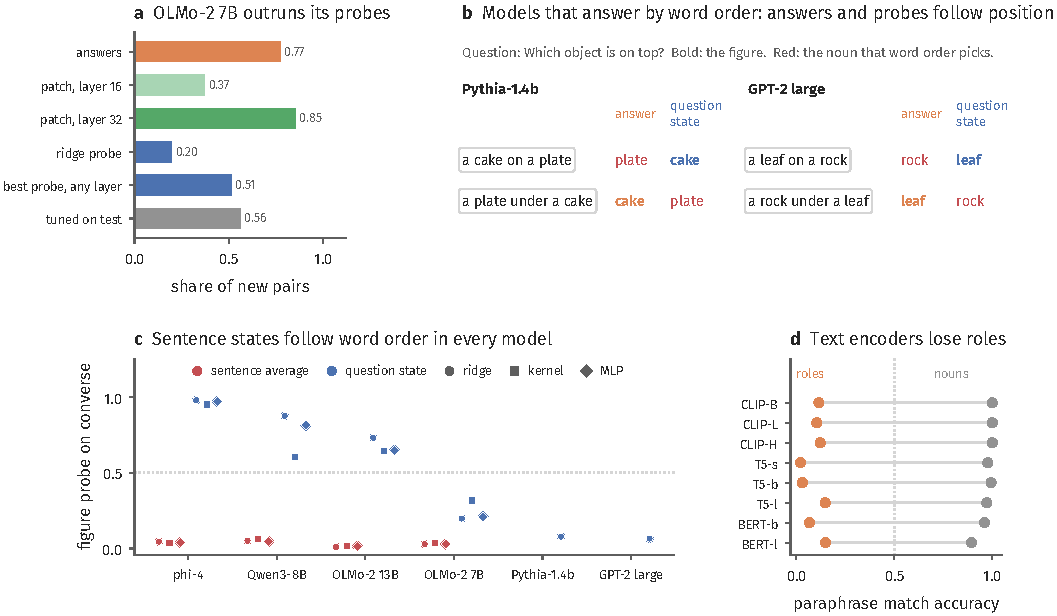
\includegraphics[width=\linewidth]{fig_weak.pdf}
  \caption{\textbf{Behavior can outrun a linear probe, and sentence states fail both tests.} \textbf{a.} OLMo-2 7B answers by meaning (orange), and its question state carries the answer under patching (green), while ridge, kernel and MLP probes of that state miss the role (blue), even with hyperparameters chosen on the test set (grey). \textbf{b.} Pythia-1.4b and GPT-2 large answer with the last-mentioned noun, and probes of their question states return the first-mentioned noun. Bold marks the figure and red the ground. \textbf{c.} A figure probe of the average over tokens returns the noun in the figure's word position (red) in every language model and for every probe, while the same probe at the question returns the figure (blue). \textbf{d.} Text encoders tell a sentence's nouns from others (grey), yet they prefer a sentence's converse paraphrase over the same paraphrase with the nouns exchanged on only 0.02--0.15 of pairs (orange), where matching meaning scores 1. New nouns; means over 3 seeds.}
  \label{fig:weak}
\end{figure}

\textbf{Models that answer by word order fail in both places.} Pythia-1.4b answers \emph{plate} for ``a cake on a plate'' and \emph{cake} for ``a plate under a cake'', the last-mentioned noun each time (Figure~\ref{fig:weak}b). A probe of its question state returns the first-mentioned noun each time. Every Pythia and GPT-2 model answers role questions at 0.41--0.56, from 160 million to 12 billion parameters and at every checkpoint of Pythia-1.4b. Their question states transfer the role at 0.07--0.10.

\textbf{Sentence states follow word order in every model.} A figure probe of the average over tokens transfers at 0.00--0.05 in every language model, against 0.15 at initialization, so training strengthens the binding to word order (Figure~\ref{fig:weak}c). Kernel and MLP probes do no better, at 0.00--0.06. The trained states carry the figure, but through codes that change with the phrasing, so these states lack shared role codes for meaning. Text encoders fail the same way. They tell a sentence's nouns from other nouns with accuracy 0.89--1.00, yet they prefer the converse paraphrase over the noun-swapped paraphrase on only 0.02--0.15 of pairs (Figure~\ref{fig:weak}d).

\textbf{OLMo-2 7B marks the limit of a linear probe.} OLMo-2 7B answers by meaning on 0.77 of pairs, while a ridge probe of its question state transfers the role at only 0.20 (Figure~\ref{fig:weak}a). Patches show that the state carries the answer. They flip 0.37 of answers at layer 16, where we fit the probe, and 0.85 at layer 32. Ridge, kernel and MLP probes at layers 16 to 32 transfer at most 0.51, and 0.56 with hyperparameters chosen on the test set. The answer thus depends on a role code that none of our probes reads, so H1 fails for these probes in OLMo-2 7B. Observation~\ref{prop:subset} still holds for a probe that contains the model's own later layers. Recoverability therefore depends on the kind of probe we fix.

\textbf{The question state serves as an embedding.} We read the question state at the end of two questions, one asking for the figure and one for the ground, and use the pair as a sentence embedding. With no fitted probe, this embedding places the converse paraphrase nearer than both role reversals for 100\% of pairs of new nouns in phi-4, 92\% in Qwen3-8B and 83\% in OLMo-2 13B (Figure~\ref{fig:decomp}d). The same embedding fails in Pythia-1.4b and GPT-2 large, whose answers follow word order.

\begin{table}[t]
  \caption{\textbf{Reading through the state repairs the failing procedures of glyph networks and recursive composers, and gives language models a sentence embedding that carries the role.} Values are $R^2$ of the system's output for the glyph and recursive networks, and the share of pairs of new nouns whose converse paraphrase is nearer than both role reversals for the language models. Each row compares runs within one experiment. Glyph values average MLP, CNN and role--filler networks over 5--9 seeds, and the sequence of 32 glyphs starts from networks trained on 16 glyphs. Recursive values use width 256, 5 seeds and 20{,}000 training steps, which give 0.27 at depth 3 against 0.26 after 6{,}000 steps in the text, and language-model values use 3 seeds.}
  \label{tab:remedies}
  \centering\small
  \begin{tabularx}{\linewidth}{@{}P{0.25\linewidth}P{0.24\linewidth}YY@{}}
    \toprule
    Repair & Failure it targets & Without & With \\
    \midrule
    Train a new decoder on a frozen state & Decoder fails on new glyphs & 0.25 & 0.75 \\
    Learn parts from single parts & Decoder fails on new glyphs & New glyph alone $-0.30$, new pair 0.26 & 0.88 and 0.47 \\
    Add parts by writing vectors & Fine-tuning forgets old pairs & Old pairs 0.18 after 32 glyphs & Old pairs 0.99; new glyph in a new role 0.71 \\
    Train the decomposer with its composer at each depth & Decomposer fails one level deeper & $0.27$, $-0.08$, $-0.29$ at depths 3--5 & 1.00, 1.00, 0.97 \\
    Read the role from two question states & The token-averaged sentence state follows word order & Paraphrase nearest for no pair & 1.00 phi-4, 0.92 Qwen3-8B, 0.83 OLMo-2 13B \\
    \bottomrule
  \end{tabularx}
\end{table}

\subsection{Where recoverability comes from}
\label{app:origins}

A state can hold its parts because the input already held them, because the architecture keeps them apart, or because training put them there. We compare each state with its input and with the same architecture under random weights (Figure~\ref{fig:origins}). For the glyph networks we add \emph{entangled inputs}, which pass each whole through a fixed random map before the encoder, three rounds of an orthogonal rotation and $\tanh$ at gain 4.

\begin{figure}[t]
  \centering
  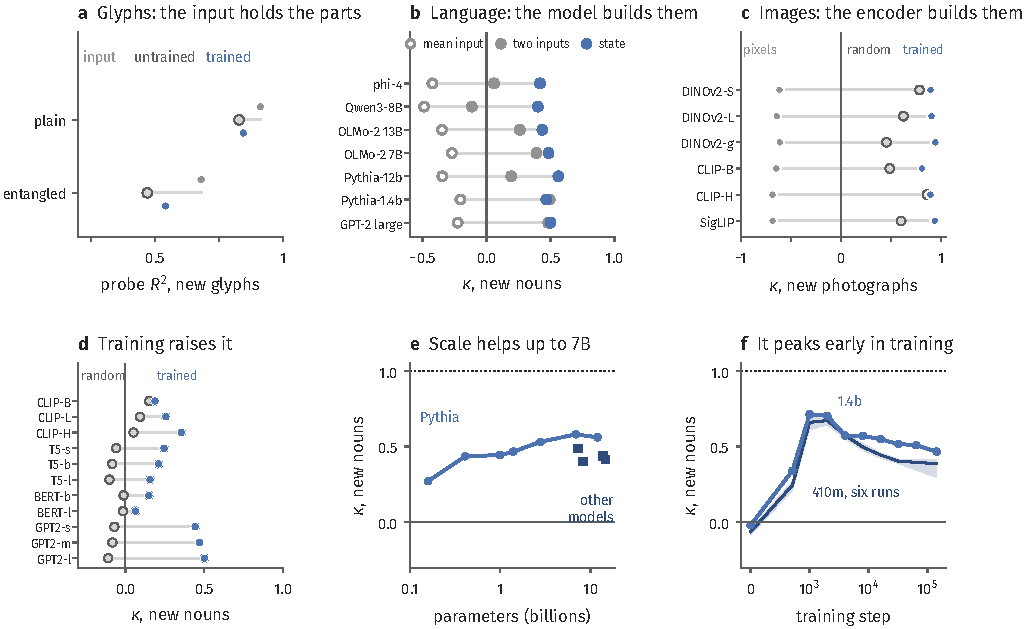
\includegraphics[width=\linewidth]{fig_origins.pdf}
  \caption{\textbf{The input supplies recoverability in the glyph networks, whereas pretrained models build it beyond their inputs.} Each row compares a trained state (blue) with its input (grey) and with random weights (light grey). \textbf{a.} Probes of new glyphs at $V = 8$, on plain inputs and on inputs entangled by a fixed random map. \textbf{b.} Language models against the average and the concatenation of the two nouns' input embeddings. \textbf{c.} Image encoders against raw pixels, scored with each encoder's own part vectors. \textbf{d.} Text encoders. \textbf{e.} Pythia models of growing size, whose scale trend is Pythia's alone, and four other language models (squares). \textbf{f.} Training of Pythia-1.4b, where step 0 is the initialization, and of Pythia-410m from six random seeds (line and range). Probes in \textbf{b} and \textbf{d}--\textbf{f} recover the nouns in their order of mention. $\kappa$ is 1 for the concatenation of the part vectors (dotted) and 0 for their sum. Means over 3--5 seeds.}
  \label{fig:origins}
\end{figure}

\textbf{Glyph networks inherit recoverability from their input.} The input pixels reach $R^2 = 0.91$ and untrained networks 0.82--0.83, and a frozen untrained encoder even supports an equally good new decoder, at 0.75 (Figure~\ref{fig:origins}a). Training in these small networks therefore mostly shapes the decoder. A fixed random map that entangles the input lowers the input's own probe to 0.68. The MLP, CNN and role--filler networks then reach $R^2 = 0.54$--$0.55$, which is 0.06--0.08 above untrained encoders and 0.13--0.15 below the input. No condition we tried lifts a state above its input. Recovery predicts the output of a new decoder, with $r = 0.98$ on entangled inputs.

\textbf{Pretrained models build recoverability beyond their input.} Averaging a sentence's input embeddings gives $\kappa = -0.21$ to $-0.49$ for the nouns in their order of mention across seven language models (phi-4, Qwen3-8B, OLMo-2 13B and 7B, Pythia-12b, Pythia-1.4b and GPT-2 large), below the sum of the part vectors. Concatenating the two nouns' input embeddings, which grants each noun's location, gives $-0.12$ to 0.49. States averaged over tokens exceed this baseline in five of the seven models and match it in GPT-2 large and Pythia-1.4b (Figure~\ref{fig:origins}b). For photographs, raw pixels give $\kappa = -0.61$ to $-0.69$ against the encoder's part vectors, which no linear map reaches from pixels, far below the quadrant states at 0.81--0.94 and below random weights at 0.29--0.72 across the encoders (Figure~\ref{fig:origins}c). Because raw pixels cannot reach semantic part vectors by construction, the comparison with random weights carries the claim for images.

\textbf{Training builds recoverability of the nouns in their positions, and Pythia's scale trend runs up to about 7 billion parameters.} Among the text encoders, the GPT-2 models reach $\kappa = 0.44$--$0.50$, CLIP-H 0.36 and the others 0.06--0.26, against $-0.11$ to $0.15$ under random weights (Figure~\ref{fig:origins}d). Within Pythia, $\kappa$ rises from 0.27 at 160 million parameters to 0.56--0.58 at 6.9 and 12 billion and levels off between those two sizes, while Qwen3-8B, OLMo-2 and phi-4 reach 0.40--0.49 and show no scale trend of their own (Figure~\ref{fig:origins}e). Pythia-1.4b peaks at 0.71 after 1{,}000 steps, 0.7\% of training, and then declines to 0.47. Six runs of Pythia-410m peak at about the same point (Figure~\ref{fig:origins}f). These probes recover the nouns in the order of mention, as the next paragraph shows, so these values score positional binding and leave the role by meaning to Section~\ref{sec:behavior}.

\textbf{Word order and architecture supply part of it.} Causal attention keeps the tokens of the first noun from seeing the second, so random weights in GPT-2 and CLIP already recover the first-mentioned noun alone with $\kappa = 0.50$--$0.58$, while the second falls to $-0.26$ to $-0.75$ and the average over roles stays at $-0.11$ to $0.15$. The control ``a $x$ and a $y$'' gives the same $\kappa$ as the asymmetric relations in every encoder, so these probes recover the nouns in their order of mention, which is a positional binding. In image encoders the choice of state decides recovery. Trained encoders reach $\kappa = 0.17$--$0.49$ in their states averaged over patches and 0.81--0.94 in their quadrant states, because the patch states keep two photographs apart whereas the average over patches blends them.
